
%=========================Introduction====================================
\section{Introduction}
A lot of numbers are usually used to describe the career of a coach in different sports: total years, matches, victories, winning percentage, champoinships, and so on. There also exist other factors that cannot be directedly obtained by these simple data, or even cannot be reflected by \textbf{any} data. These facts make it almost impossible to propose a perfect assessment method for college coaches.



Our goal is to build a mathematical model to find the best all time college coach or coaches in the previous century in certain sports. Here we mainly focus on NCAA Men's basketball, football,

In our metrics for assessment, we use 4 parameters

We develop 2 parameters that can reveal the ability of a coach. Promotion   Stability      Our metric attaches high importance to these aspects.   based on the performance of the team he is managing inside the conference it belongs to
%Assessing a college coach can be hard. Traditionally, the assessment of a coach is entirely decided by the  performance of his team. This method, however, is not convincing enough in that it neglects the promotion a coach has brought to his team.

We, on the other hand, develop a model trying to combine these two aspects together by taking both these two elements, performance of the team and promotion brought by the coach, into consideration. Furthermore, we develop a method to evaluating the performance of a team with limited information, which makes the evaluation for coaches of the whole past century possible since data in those early years may not be as comprehensive as it is now.



%=============================Model framework==========================================
\section{Framework of the Model}
Basically, our model assesses a coach based on the performance of teams.











In order to find the promotion and stability of a coach, a fundamental issue here is to properly evaluate the performance of a team in a season. This issue, however, is related to several aspects which are intricately connected with each other. Based on the competetion system of NCAA, our model develops a method to give an assessment of the performance for the team based on its Win-Loss percentage in the regular season inside the conference it belongs to     , its opponents' strength and the strength of conference it is in.






In the evaluation of the performance of a team in a single year, we consider its matching results in the regular season, and also estimate the overall strength of this conference and the intensi

Based on a comprehensive evaluation of performance for all teams, the model get some parameters which can depict different aspects of a coach. These parameters are carefully selected such that they are independent of each other and each parameter is well related to an aspect of the coach. Besides, these parameters will make full use of our data found, which suggests the comprehensiveness of our model.

A series of preliminaries are set to filter coaches ahead of the model in order to minimize our size of candidates. These preliminaries are selected such that real "legends" will not be overlooked and will sure to be selected. This procedure will greatly alleviate our calculation, thus making more comprehensive and complicate model possible.

The model can be explained by \textbf{Figure 1}:
\begin{figure}[!ht]
\centering
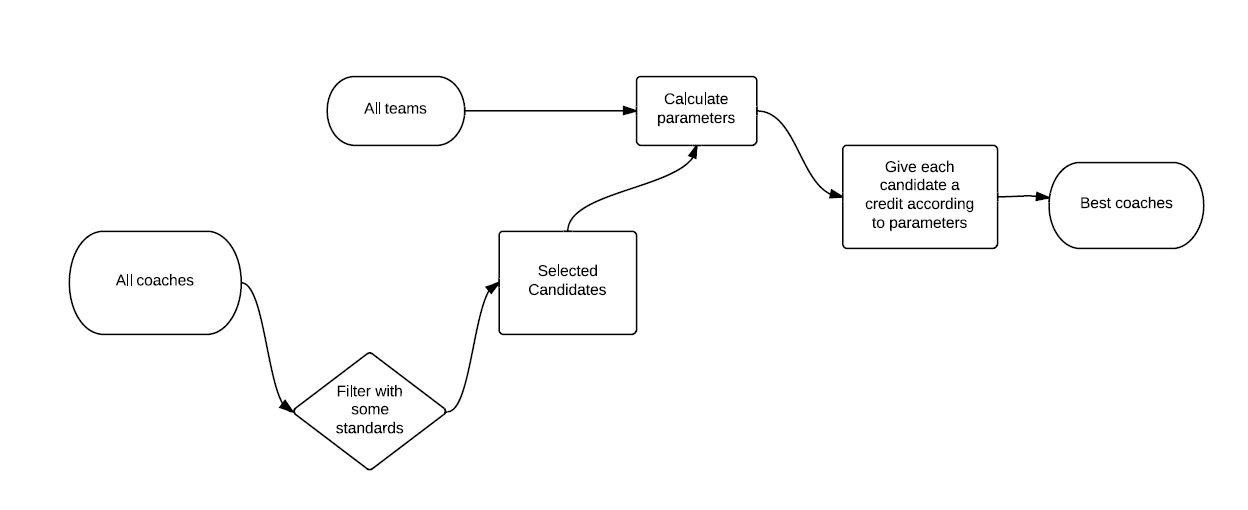
\includegraphics[width = 150mm]{picture/OverallFrame.png}
\caption{Overall framework}
\end{figure}

In the model, based primarily on records of NCAA teams for the last century, we synthesize the data into two parameters: performance and promotion.

Performance measures the team's performance during the time directed by the coach of interest. This parameter is similar to the traditional way of measurements. Promotion measures to what extent did the coach enhanced the performance of the team. As will showed later, these two parameter is based on data of different periods of a team, so they do depict different aspects of a coach.

\section{Basic definitions}

\subsection{Win-Loss percentage}
Since the model's purpose is to rank coaches in the past century, records must be carefully selected to enable the comparison between teams from different era. We select Win-Loss percentage(WLP) as one of its basic figures.
\newtheorem{definition}{Definition}
\begin{definition}
Given a season of interest, suppose the team under consideration has $w$ wins, $l$ losses. The Win-Loss percentage(WLP) is:
$$WLP \doteq \frac{w}{w + l}.$$
\end{definition}

The selection is based on the following considerations:

\begin{itemize}
\item Win-Loss percentage for the sports we select is recorded or can be easily calculated throughout the whole past century.
\item Win-Loss percentage can minimize the influence brought by different tournament system and different rules, which provides the model with more generality.
\item For all teams, the Win-Loss percentage is of the same scale, which means $WLP\in [0,1]$.
\item The expectation for Win-Loss percentage is the same for all teams, which is 0.5. So this is a fair index when comparing performances across teams, avoiding prejudices brought by the model.
\end{itemize}

\subsection{Conference Strength}
Besides records for a single team, the model also considers the strength of the conference the team is in. By this number we estimate the overall strength of teams in a conference and can be used to compare teams from different conferences.
\begin{definition}
In a season of interest, the teams in a conference have a total of $W$ wins, $L$ losses, $D$ ties against the teams from other conferences. Then its \textbf{Conference Strength} $p$ is
$$p = \frac{W}{W+L}.$$
\end{definition}

%Here overall wins(losses, ties) means all games, whether the opponents are from the same conference or not, is taken into consideration, and conference wins(losses, ties) only considers those games with opponents in the conference.

Note that it is similar to the definition of WLP, so this parameter has similar properties as WLP:
\begin{itemize}
\item Conference Strength for the sports we select can be calculated throughout the whole past century.
\item Conference Strength is related to the overall performance of teams in a conference, and does not necessarily related to tournament system and rules, which provides the model with more generality.
\item For all conferences, Conference Strength is of the same scale, which means $p\in [0,1]$.
\item The expectation for Conference Strength is the same for all conferences, which is 0.5. So this is a fair index when comparing performances across conferences, avoiding prejudices brought by the model.
\end{itemize}

%==================================��������==============================================

\subsection{Measurement for Performance}
In this part, we will explain the method to measure a team's performance. This number will serve as a basic part for evaluating promotion and stability. For the team, we're interested in its WLP of all conference games in the regular season.

\newcommand{\performance}{x_i\frac{1+b(p-0.5)}{1+a\sigma}}
\begin{definition}
In a season of interest, suppose there are N teams in a conference $t_1, t_2,\dots,t_N$. Team $t_i$ has a WLP $x_i$. The conference has a Conference Strength $p$. Then the performance for team $t_i$ is
$$y_i\doteq \performance.$$
\end{definition}

Here $\sigma$ is the standard deviation of $x_1, x_2, \cdots, x_N$, which is $\sigma = \sqrt{ \frac{\sum_{i=1}^{N}(x_i - \mu)^2}{N}}$ and $\mu = \frac{\sum_{i=1}^N{x_i}}{N}$. Thus $\sigma$ is used to estimate the intensity of competition inside this conference. The smaller $\sigma$ is, the more intense is the inner competition.

In the definition, $a$ and $b$ are both tunable positive parameters and both should be relatively small. %In fact, here $a$ depicts the influence of the team's opponents and $b$ depicts the influence of the conference.

The definition of $y_i$ has the following properties:

\newtheorem{property}{Property}

\begin{property}
$$\frac{\partial{y_i}}{\partial{x_i}} > 0$$
\end{property}
\begin{comment}
\begin{proof}
$$\frac{\partial{y_i}}{\partial{x_i}} = \frac{1+b(p-0.5)}{1+a\sigma}$$
Since both $a$ and $b$ are positive, we have $\frac{\partial{y_i}}{\partial{x_i}}>0$.
\end{proof}
\end{comment}

\begin{property}
$$\frac{\partial{y_i}}{\partial{\sigma}}<0$$
\end{property}
\begin{comment}
\begin{proof}
$$\frac{\partial{y_i}}{\partial{\sigma}} = -x_i\frac{1+b(p-0.5)}{1+a\sigma}\ln(1+a\sigma)$$
Similarly, we have both $a$ and $b$ are positive, so $\frac{\partial{y_i}}{\partial{\sigma}}<0$
\end{proof}
\end{comment}

\begin{property}
$$\frac{\partial{y_i}}{\partial{p}} > 0$$
\end{property}
\begin{comment}
\begin{proof}
$$\frac{\partial{y_i}}{\partial{\p}} = \frac{b}{1+a\sigma}x_i > 0$$
\end{proof}
\end{comment}

These three properties are easy to observe and they suggest how performance is related to three variables. Then the team's performance is based on its WLP, and should be scaled up with the increase of the conference strength and intensity. Specifically, since $p=0.5$ means the conference is of average level among all conferences, there is a $(p-0.5)$ inside the definition to be consistent with this property.


We choose appropriate values for $a$ and $b$ to make this measurement be consistent among all conferences and all eras. The expectation of $y_i$ is close to 0.5 given that $a$ and $b$ are both small. So $\sigma$ and $p$ will not bring into the model too much prejudices but only minor amendments.


%Next we have \textbf{Property 4}, which will guarantee the comparable between different teams from different conferences or/and different eras.
%\begin{property}
%$$\frac{\sum_{i=1}^N{y_i}}{N}<\frac{1-b}{2(1+a)}$$
%\end{property}

%To prove \textbf{Property 4}, first we prove the following claim:
%\newtheorem{claim}{Claim}

%\begin{claim}
%In a tournament with N teams $t_1,t_2,\dots,t_N$, team $t_i$ has a WLP $x_i$, then
%$$\sum_{i=1}^N{x_i} = \frac{N}{2}$$
%\end{claim}
%\begin{proof}
%Each team plays the same number of games, which is $2N\choose 2=N(N-1)$, suppose team $t_i$ has $w_i$ wins and $d_i$ ties. Then
%$$x_i=\frac{w_i + 0.5t_i}{N(N-1)}$$
%so
%$$\sum_{i=1}^N{x_i} = \frac{\sum_{i=1}^N(w_i + 0.5t_i)}{N(N-1)}$$
%Since each game is counted either as a win and a loss or as two ties, we have
%$$\sum_{i=1}^N(w_i+0.5t_i)=\frac{N(N-1)}{2}$$
%so we have
%$$\sum_{i=1}^N{x_i} = \frac{N}{2}$$
%\end{proof}

%Then we can prove \textbf{Property 4}
%\begin{proof}
%\begin{align}
%\sum_{i=1}^Ny_i &= \frac{1+b(p-0.5)}{1+a\sigma}\sum_{i=1}^Nx_i\\
%&=\frac{1+b(p-0.5)}{1+a\sigma}\frac{1}{2}\\
%&<\frac{1-b}{2(1+a)}
%\end{align}
%\end{proof}

\textbf{Comparison with SRS}

Here we compare our measurements with another system of performance measurement called simple ranking system(SRS), which is used for ranking college basketball teams recently in National Collegiate Athletic Association(NCAA).

SRS is aimed at involving opponent's performance into a single team's assessment and finally make reliable predictions about which team will get the most credits in the conference. Different from our model, SRS builds its evaluation on a set of equations
\begin{align}
\nonumber
&R_1 = x_1 - \mu + \frac{1}{N-1}\sum_{j\neq i} R_j\\\nonumber
&R_2 = x_2 - \mu + \frac{1}{N-1}\sum_{j\neq i} R_j\\\nonumber
&...\\\nonumber
&R_N = x_N - \mu + \frac{1}{N-1}\sum_{j\neq i} R_N \\\nonumber
\end{align}
where $\mu = \frac{\sum_{i=1}^Nx_i}{N}$

This set of equations can be solved with Gauss-Seidel algorithm. Obviously, there are two parts in each equation. The first one is $x_i - \mu$, which stands for credits got by the team. Another part is  $\frac{1}{N-1}\sum_{j\neq i} R_j$, which can be seen as an amendment brought by its opponents.

This method, however, cannot achieve its initial purpose. Further study shows that this set of equations has a solution set like
$$R_i = \frac{N-1}{N}x_i + c$$
where $c$ is an arbitrary constant.

So what we got from this method only relies on N and $x_i$, instead of $x_1, x_2,\dots,x_N$ as we wished. In contrast, our model do take every team's WLP into consideration, which suggests this method can partly shows the relationships among different teams inside the conference.

Also, our measurement takes into account the overall performance of the conference while SRS does not. So SRS cannot be applied to compare teams from different conferences.

\subsection{$PRM(c)$}
The calculations of $PRM(c)$ and $STB(c)$ are based the above definition of performance of a team in a specific season. To make it clear, we denote it by $PERF(t, s)$, where $t$ is the team, and $s$ is the season.

%The promotion is determined by two parts of data. One is the team's \emph{historical performance}, which means how this team works before the coach came to the team and another is the team's \emph{temporary performance}, which shows how the team works during the period directed by the coach. The model makes a prediction based on the historical performance and compares the prediction with its real performance. The result of the comparison will be used as promotion.
For a coach $c$, we first choose a team $t$ that he has coached. If he has only coached one team in his career, then $t$ is this team. If he has coached more than one team, we choose the one that he has coached for the longest time.

Suppose $C$ coached $t$ in seasons $s_1, s_1+1, \cdots, s_2$.

Let the average performance of $t$ in the first $r$ seasons coached by $c$ $s_1, s_1+1, \cdots, s_1+r-1$ be $P_{after}$, and the average performance of $t$ in the last $r$ seasons before $C$'s coaching be $P_{before}$. Here $r$ is a constant to be chosen. Let $PRM(c)=P_{after}-P_{before}$. To make it clear:
\begin{definition}
$$PRM(c)= \frac{\sum_{i = 1}^{r}PERF(t, s_1+i-1)}{r}-\frac{\sum_{i = 1}^{r}PERF(t, s_1-r)}{r}.$$
\end{definition}

%\begin{definition}
%Suppose we have a team's historical performance $y_1, y_2,\dots, y_s$ and its temporary performance $y_{s+1}, y_{s+2},\dots, y_r$. Then the promotion is
%$$p\doteq \frac{\sum_{i = s+1}^ry_i}{r-s} - \frac{\sum_{i=1}^sy_i}{s}$$
%\end{definition}

This definition of promotion is straightforward. This difference descibes the promotion that the coach brought to this team.

Note that when calculating $PRM(c)$, a lot of information is used other than those are obviously related to $c$, which suggests the model is more comprehensive. Since the data we can use are limited because of the long time interval, taking full use of data is an advantage of our model.

\subsection{$STB(c)$}
\begin{definition}
Let $STB(C)$ be the standard deviation of $PERF(t, s_1), PERF(t, s_1+1), \cdots, PERF(t, s_2)$.
\end{definition}

This is also easy to understand. We use the standard deviation of the team's performances to estimate $STB(c)$.
%===============================�ۺϷ���============================================
\section{Synthesized Evaluation Based on Four Aspects}
In this section, we will give an overall credit for a coach based on his performance in four aspects discussed in previous section. For a coach c, $PRM(c)$, $STB(c)$, $ACH(c)$ and $WLP(c)$ will be summed up with weights decided by analytic hierarchy approach.

The hierarchy for this problem is shown in \textbf{Figure 2}
\begin{figure}[!hf]
\centering
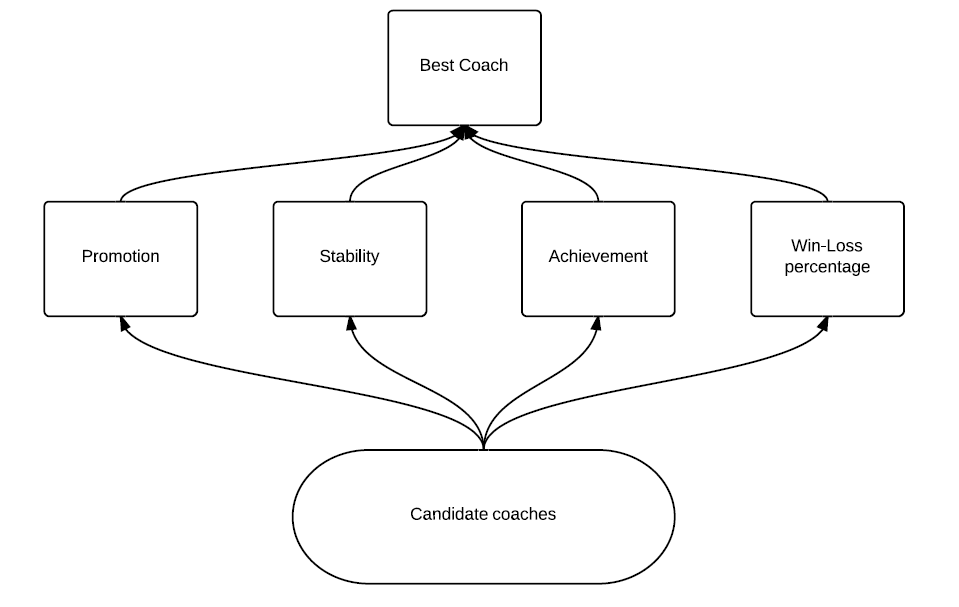
\includegraphics[width = 150mm]{Hierarchy.png}
\caption{Hierarchy}
\end{figure}

Based on this hierarchy, we have the following comparison matrix
$$
\left(
  \begin{array}{cccc}
    1 & \frac{1}{3} & \frac{1}{7} & \frac{1}{5} \\
    3 & 1           & \frac{1}{3} & \frac{1}{3} \\
    7 & 3           & 1           & 3           \\
    5 & 3           & \frac{1}{3} & 1           \\
  \end{array}
\right)
$$

Now we verify the matrix
\begin{align}
CI &= \frac{\lambda_{MAX}(A) - 4}{3}\nonumber\\
\lambda_{MAX} &= 4.13973 \nonumber\\
RI &= 0.90\nonumber
\end{align}

So $CR = \frac{CI}{RI}=0.052 < 0.1$, the matrix can be used as comparison matrix.

Then we have its eigenvectors is $(0.056, 0.139, 0.525, 0.280)^T$.

Now we have the synthesized credit defined as following

\begin{definition}
For a coach $c$, the synthesized credit is
$$EVA(c) = 0.056PRO(c) + 0.139STA(c) + 0.525ACH(c) + 0.280WLP(c)$$ 
\end{definition}

Actually, there are many choices for comparison matrix here and thus the definition of $EVA$ is not unique. The definition of $EVA$ varies as the whole evaluation system focusing on different aspects of a coach. Here we pays more attention to achievement and overall win-loss percentage. One may get a different result if he focus more on the former two aspects.

Analytic hierarchy process here offers a systematic way to decided the weight based on the focus of the evaluation system. Compared with setting these weights empirically, this method provides a guideline and thus providing a more reliable model.

%========================ģ�ͽ��============================

\section{Result}
\indent Records in terms of achievement, stability, average performance, and
promotion are generated by computer programs. These data are
summarized in the following four histograms.\\
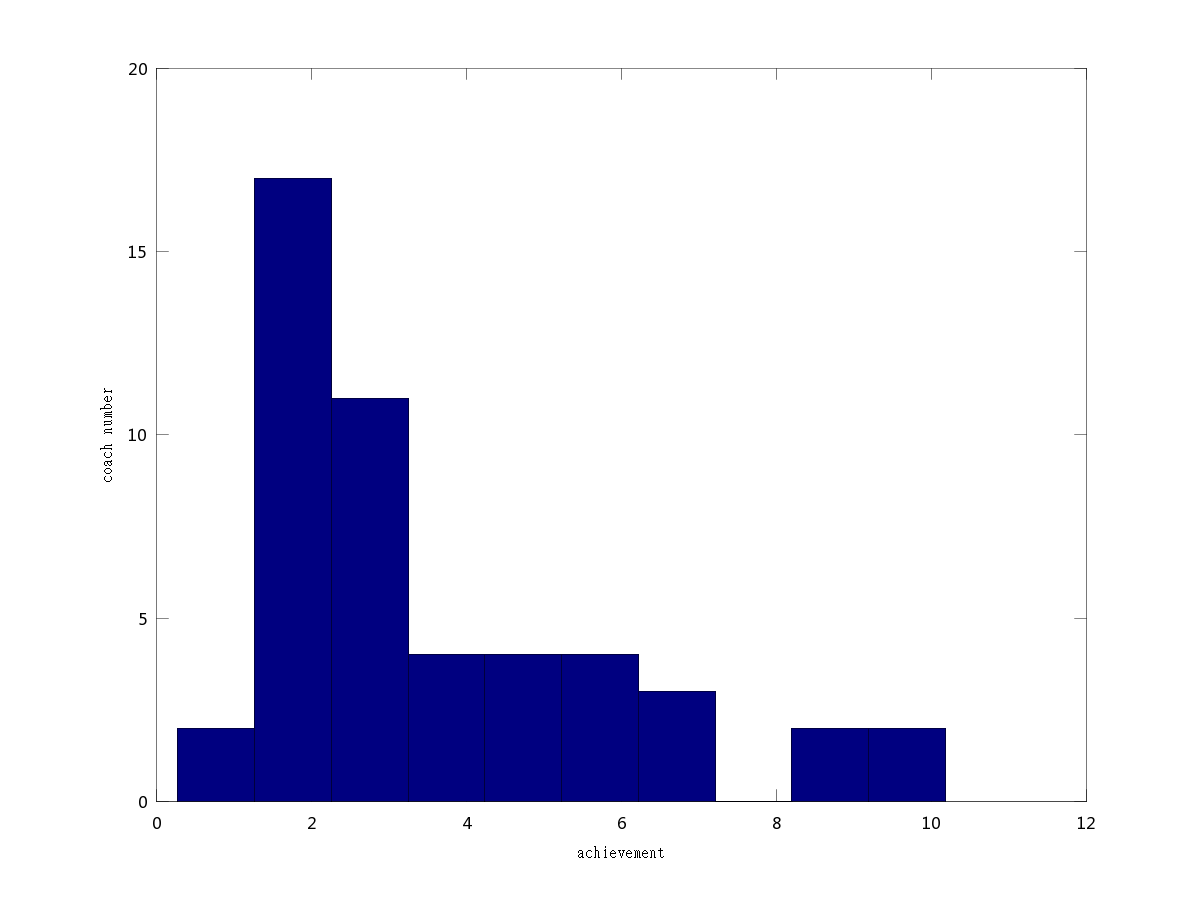
\includegraphics[width=2.5in, height=2.5in]{ach}
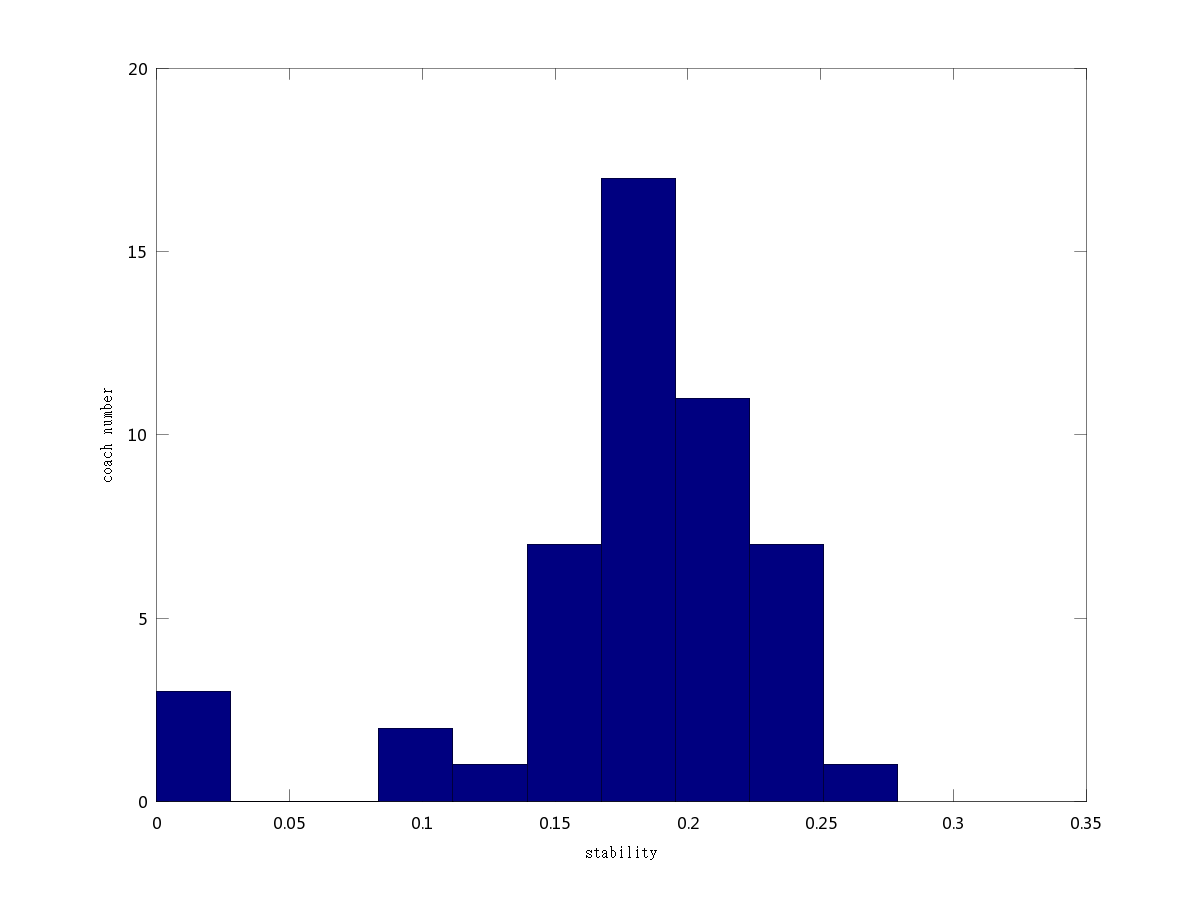
\includegraphics[width=2.5in, height=2.5in]{sd}\\
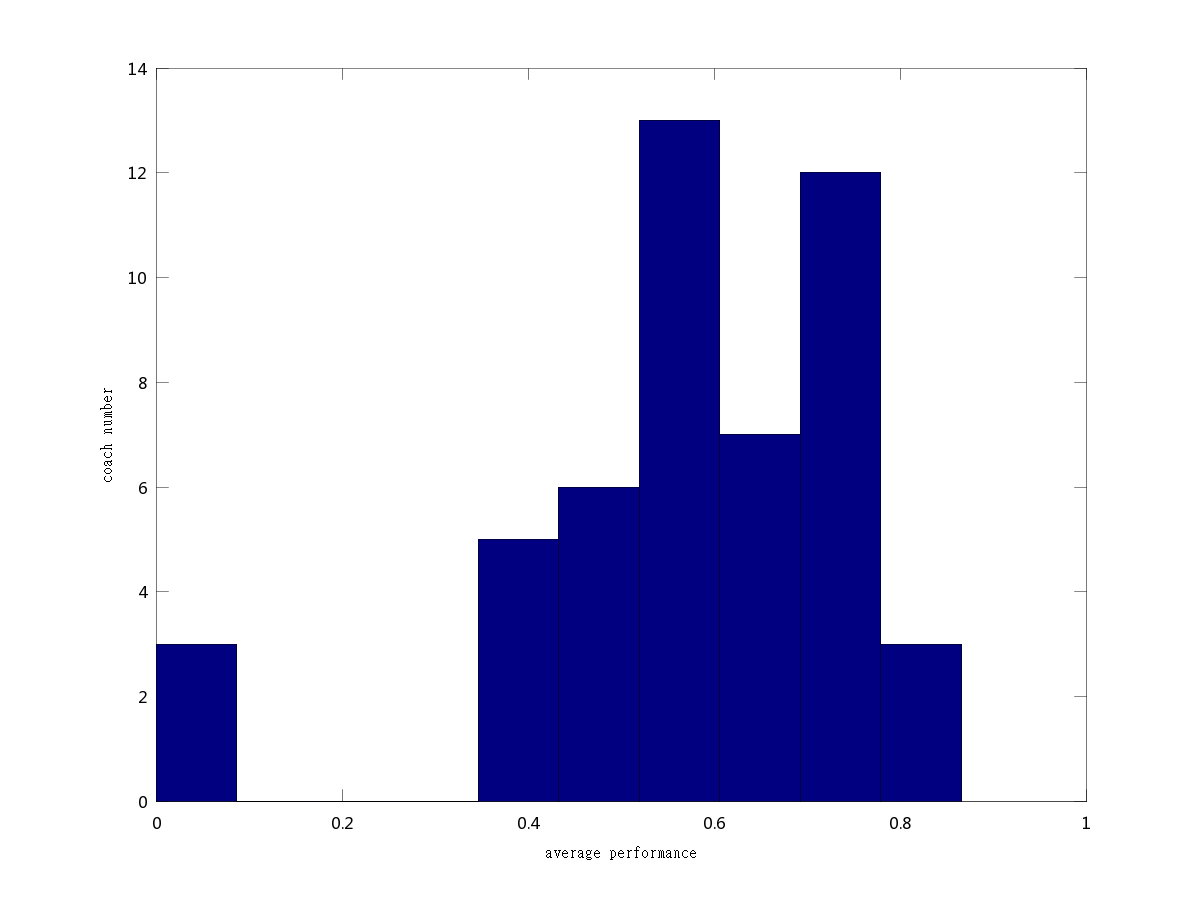
\includegraphics[width=2.5in, height=2.5in]{average}
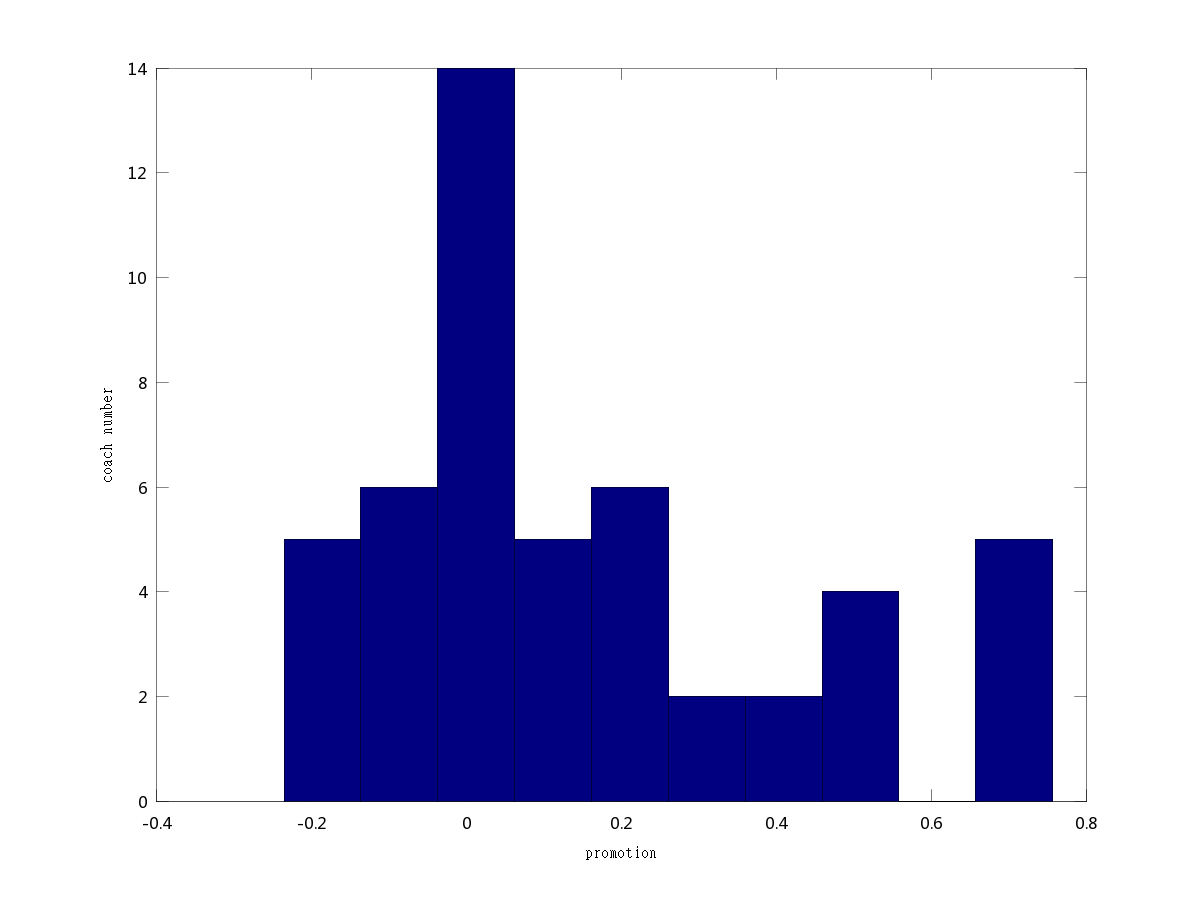
\includegraphics[width=2.5in, height=2.5in]{margin}\\
\indent By applying the Analytical Hierarchy Model, we can obtain the
evaluation of each one of the top-50 candidates. Distribution of the
scoring is showed by the next histogram.\\
\begin{centering}
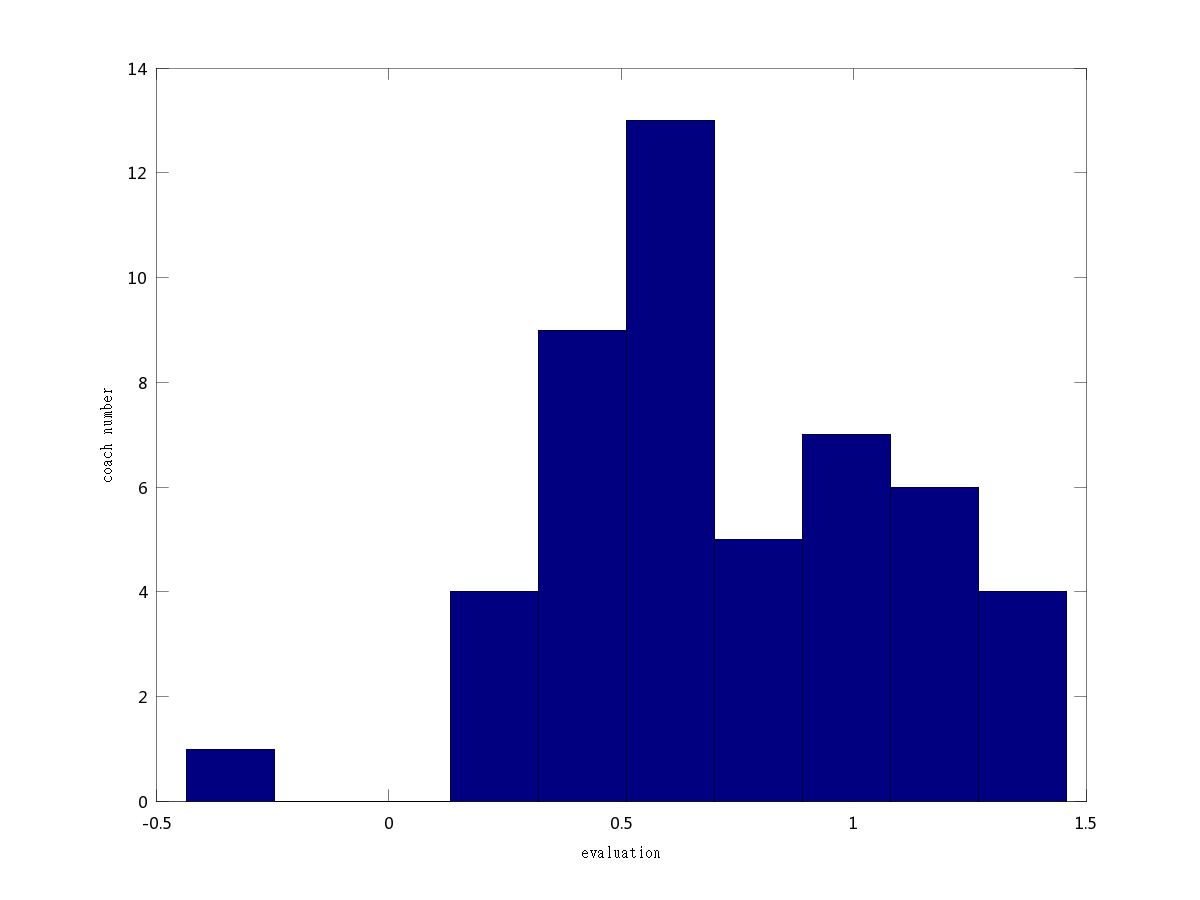
\includegraphics[width=2.5in, height=2.5in]{eva}\\
\end{centering}
\indent Sorting the values in a descending order, we eventually reveal
the names of the top-5. They are, \textbf{John Wooden}, \textbf{Mike
  Krzyzewski}, \textbf{Adolph Rupp}, \textbf{Dean Smith},
\textbf{Denny Crum}.\\

\section{Conclusions}
\indent The list of our top-5 basketball coaches seems reasonable
since three of the five winners are within the top-10 of our 50
candidates, otherwise we would have to question why our model should
have blocked out so many widely recognized coaches. But fortunately,
these our model produces a moderate result. One exception is that
\textbf{John Wooden} who ranked 25, somewhat behind other top-5
winners, won the first place. A fair deduction is that in the
Analytical Hierarchy model, achievement is given most credit, and
since \textbf{John Wooden} has secured a largest number of NCAA
champion, he might have gained some advantages at that
point. This suggests that we can modify Analytical Hierarchy Model
parameters to expect different results.

\section{A Summary}
\indent In this paper, we devise a model to distinguish 5 top
basketball coaches out of all the coaches in the last 100 years. We
formulate four aspects that determines our final decision. They are
\textbf{achievement}, \textbf{performance}, \textbf{stability}, and
\textbf{promotion}. After that, an Analytical Hierarchy Model plus
methods of regularization is adapted to synthesize our four aspects to
obtain an eventual evaluation of a coach.\\\\
\indent In order to test the effectiveness of our model, we make an
comparison between the measurement of SRS index and our team
performance curve, which reinforce reliability of team performance as
one of the main aspect we consider.\\\\
\indent Before applying our model to concrete data, we narrow our
candidates by lower-limit of total wins in career to a set of 50
coaches to make life easier.\\

%================================ģ������==============================
\section{Evaluation of the Model}
In this part, we will show the model's effectiveness by showing our measurement does reflect the intrinsic ability of a coach.

First we will show the effectiveness of our measurement for a team's performance. We illustrate this by comparing our result of Kansas with SRS.

SRS, as discussed in previous section, is considered to be a metrics for performance of a team and is recorded in NCAA teams. Now we compare our performance calculated for Kansas and SRS for both Kansas and its conference, the Big 12. The result is shown in \textbf{Figure 3}.

\begin{figure}[!ht]
\centering
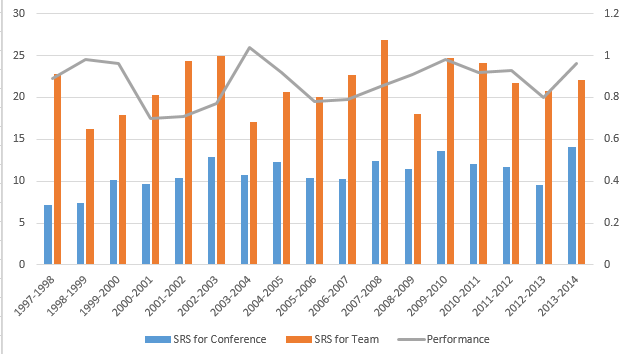
\includegraphics[width = 150mm]{Comparison.png}
\caption{Comparison between Performance and SRS}
\end{figure}

From the figure, our measurement generally follows the same tendency as SRS for the team. However, from season 1999-2000 to 2000-2001, there is a inconsistent between the two figures. Meanwhile, SRS for the conference is also inconsistent with SRS for the team. This suggests that compared with SRS, our measurement for the performance of a team takes the overall performance of the conference into consideration, and thus this measurement can be used in comparison between teams from different conferences.

There are also several other inconsistencies in the figure. These inconsistencies are due to the variance of teams in the conference, which is introduced in our model explicitly, leading to a more convincible result.

\begin{comment}
We take Princeton for example to show the effectiveness of our team performance measurement. The performance figure of Princeton is shown in \textbf{Figure 3}.
\begin{figure}[!hf]
\centering
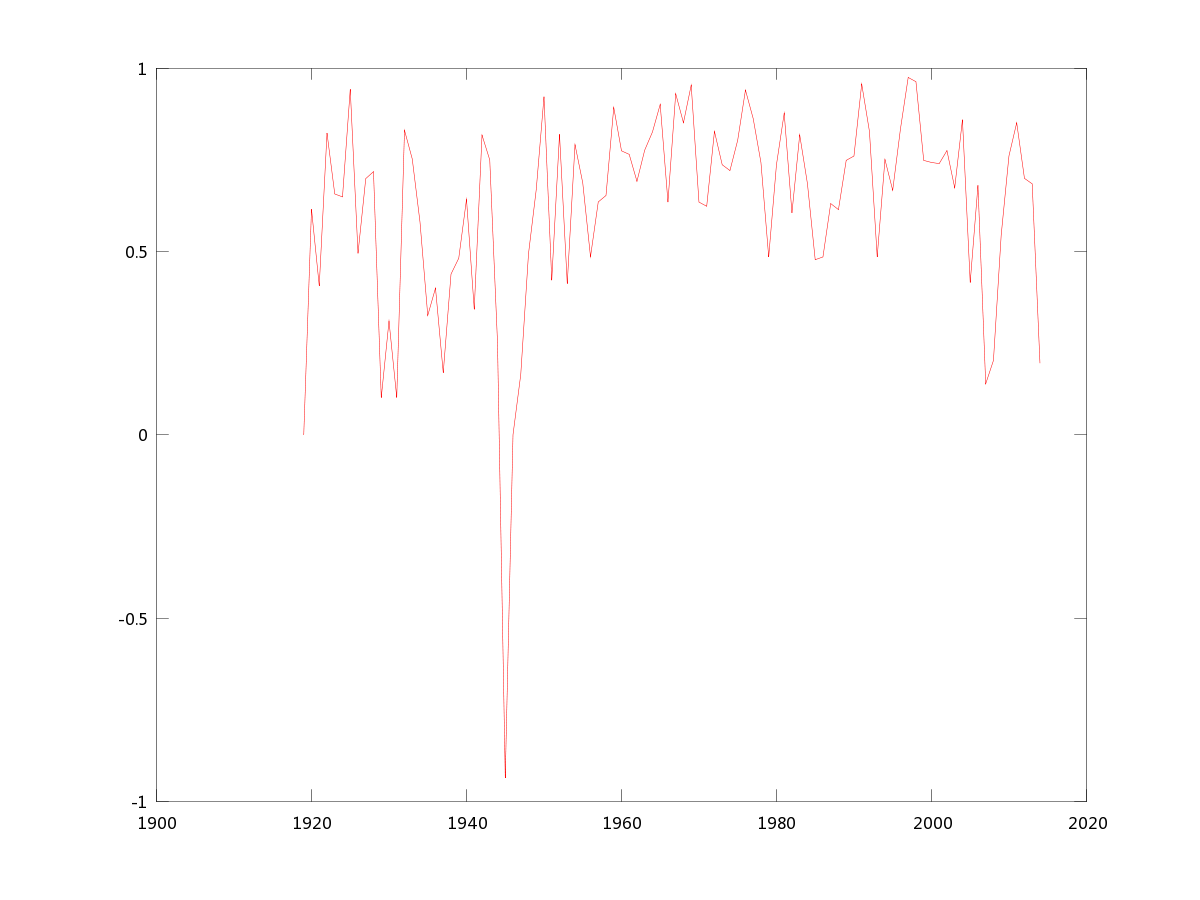
\includegraphics[width = 150mm]{Princeton.png}
\caption{Perforce of Princeton}
\end{figure}

In the figure, there is a sharp drop down at around 1945. Further investigation explains that Princeton performs badly during this period until they have a new coach in season 1946-1947.So our measurement for team performance can reflect some intrinsic factors of a team.
\end{comment}

Next, we will take two coaches, Mike Krzyzewski and Bob Knight, for example to show how the model evaluate a coach based on their coach experience. In our model, Mike Krzyzewski gets a credit of 1.38 and Bob Knight gets a credit of 1.08. Their basic information is listed below

\begin{tabular}{c|c|c|c}
  Name            & Overall WLP & Conference Champion & NCAA Champion \\\hline
  Mike Krzyzewski & 0.764       & 12 times            & 4 times       \\
  Bob Knight      & 0.706       & 11 times            & 3 times  
\end{tabular}

In this table, we see the two coaches have got almost the same championships during their coach life. Mike Krzyzewski gets a better overall win-loss percentage than Bob Knight, which is consistent with the fact that the former owns slightly more champions than the latter.

Furthermore, the performance of their team is shown in these two figures

\begin{centering}
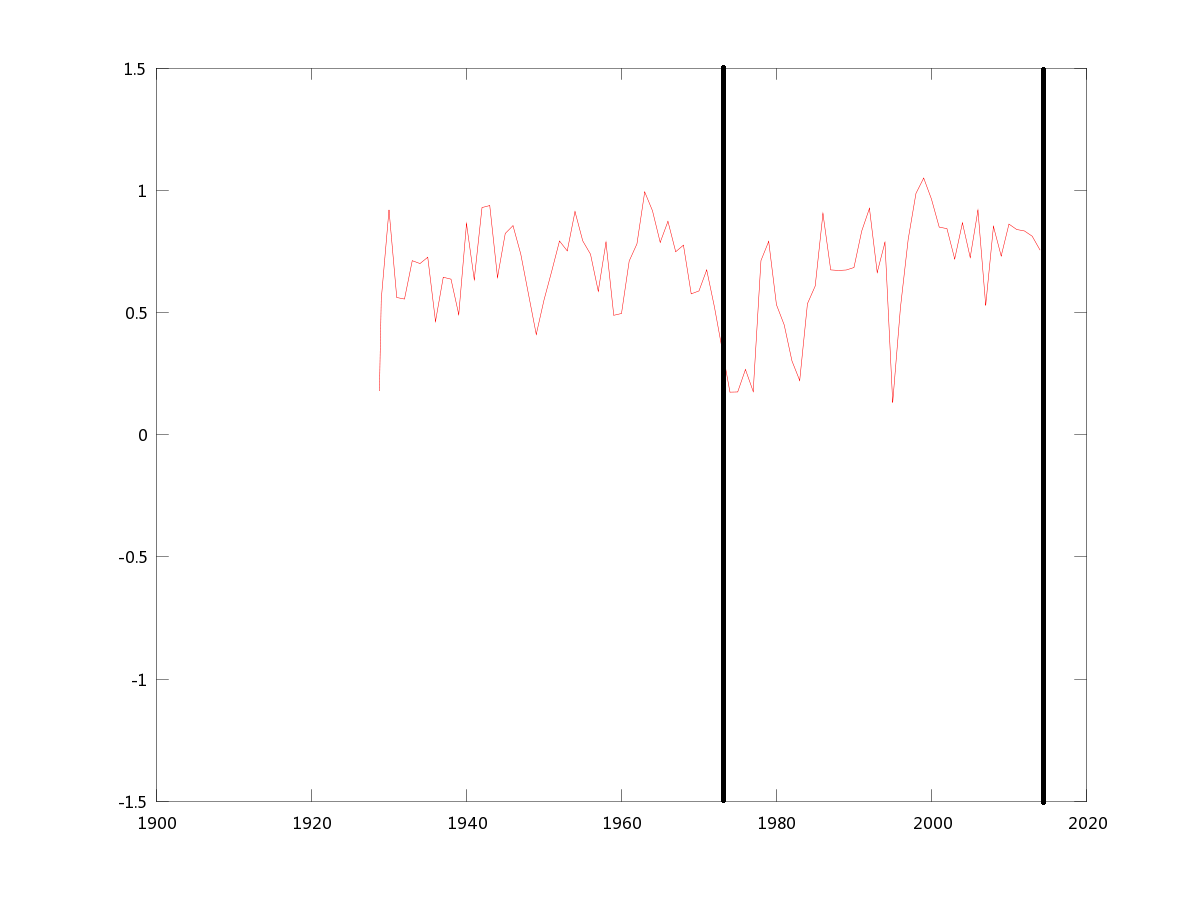
\includegraphics[width = 60mm]{Duke.png}
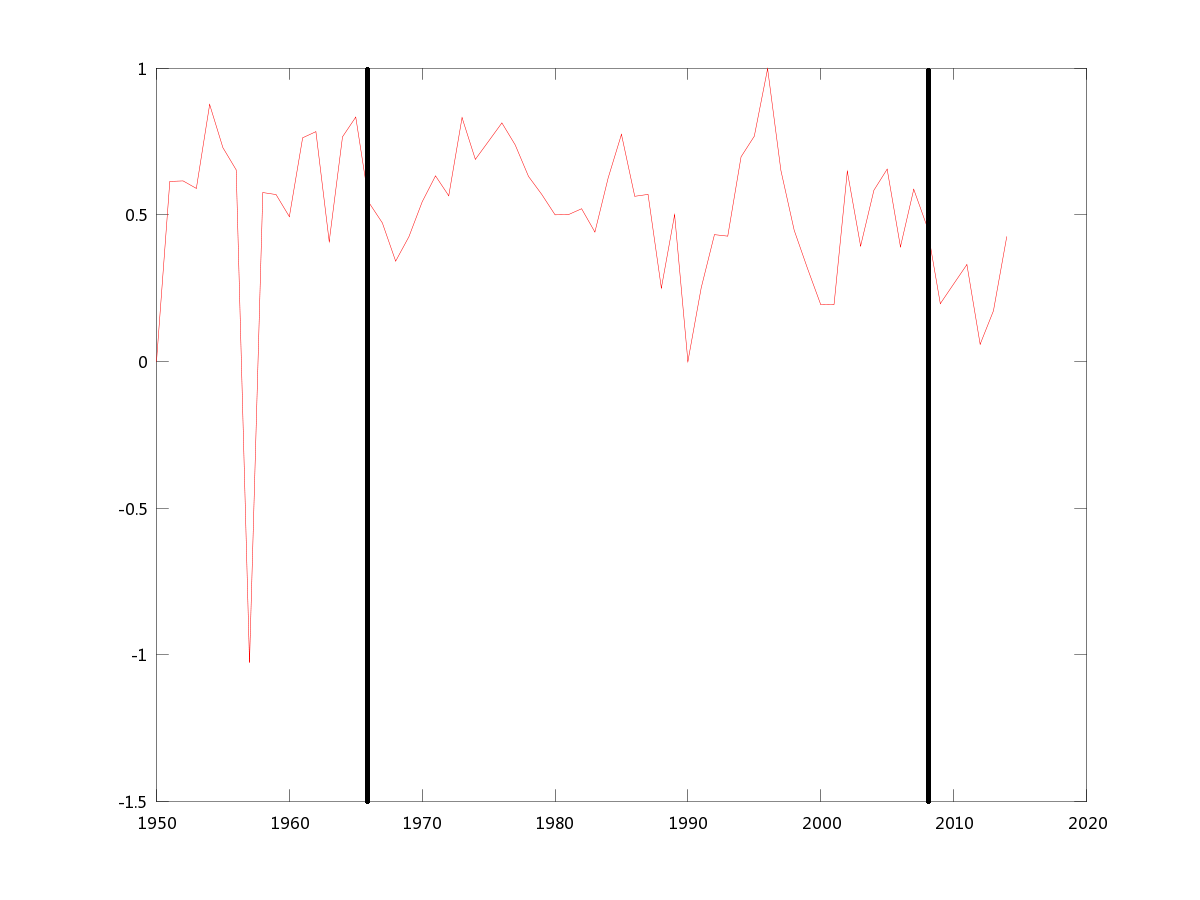
\includegraphics[width = 60mm]{Texas_Tech.png}
\end{centering} 

The left figure is performance figure for Duke where Mike Krzyzewski directed from 1976 till now. The right figure is performance figure for Texas Tech where Bob Knight directed during 1966-2008.

From the figure we can see that their teams performance does not have much difference. As for tendency, however, Duke had a significant promotion the time Mike Krzyzewski took the team while Texas Tech continued to become worse when Bob Knight joined. This comparison suggests Mike Krzyzewski has a better ability to promote the team than Bob Knight, and thus Mike Krzyzewski scores higher than Bob Knight.

With analysis provided above, we are pretty sure about Mike Krzyzewki does do better than Bob knight, which is consistent with the result of our model.

%======================================================================
\section{Strengths and weaknesses}
Like any model,the one present above has its strengths and weaknesses. Some of the major points are presented below.

%============================ģ����ȱ��====================================
\subsection{Strengths}
\begin{itemize}
\item \textbf{Applied widely}\\
The model is based on data that is accessible for most of sports, which serves as the foundation of its generality. Furthermore, the model is loosely connected to the rules of the sport under consideration. The model is built on relative performance of a team, avoiding entanglements with intricate technique details. The use of analytic hierarchy process makes possible the control of emphasis on different aspects in the evaluation. As far as sports in NCAA is concerned, the model works well. In fact, besides college sports, the model can be applied to professional conferences and tournaments with little change and the model works for both male and female sports.
\item \textbf{Dynamic}\\
The model is dynamic in the sense that data is not used individually. Not only is the overall statistics considered, but the relationship between teams and trend of a team over years contribute to the final result. This model, different from a static model where a game is evaluated individually, is more suitable for evaluating over a period of time. A dynamic model also suggests a more comprehensive use of data, which is a valuable feature with respect to the limit of data due to a time interval.
\item \textbf{Systematic}\\
The model is systematic in that it is composed of several well designed layers, each is tightly connected with an hierarchy in the evaluation. This well designed framework brings the model extendibility. When an extra element is needed to be included in the model, it will be easily embedded in because what matters is only the layer corresponding to the element. Besides, this framework make possible free control of the evaluation process. With parameters properly adjusted, the model can be transformed into another evaluation system focusing on some other aspects.
\item \textbf{Comprehensive}\\
Different from traditional evaluation system in which only team performance is considered, the model makes a comprehensive comparison, taking into consideration the difference among conferences and changes over time. Besides, these variables are properly quantized to be comparable among each other, which makes the model more reliable. 
\item \textbf{Stable}\\
Aware of the fact that coincidence plays an important role in the field of sports, we take advantage of several methods to guarantee the model is stable, minimizing the effect of coincidence. We focus on overall performance or performance over an interval of time, which will eliminate those influence remarkably. Besides, the introduction of variance will explicitly evaluate the influence of coincidence, leading to a more stable model.
\end{itemize}

\subsection{Weaknesses}
\begin{itemize}
\item \textbf{Empirical}\\
Some of parameters in the model is empirical. Some factors, such as the importance of a game, are hard to be quantized, so the model takes some empirical values. Further professional studies may be needed to support our choices or optimize them. Another way might be determining these parameters by learning. With limited time and efforts, however, we cannot give further explanations for these parameters and set them empirically.
\item \textbf{Communication skills is not considered explicitly}\\
Communication with teams can be an important responsibility for coaches. This, however, may require information got directly from teammates, which is impossible for us. Similarly, we believe various of aspects are included in a coach's responsibility besides directing the team to get good grades. The model does not consider these aspects explicitly. Further studies in this field can help with the robustness of our model greatly.
\end{itemize}



\begin{thebibliography}{99}
\addcontentsline{toc}{section}{References}
\bibitem{1} National Collegiate Athletic Association(2012). \emph{NCAA Basketball Coaching Records}. Retrived Feberary 9, 2014 from \url{http://fs.ncaa.org/Docs/stats/m_basketball_RB/2012/coaches.pdf}.
\bibitem{2} National Collegiate Athletic Association(2012). \emph{NCAA Football Coaching Records}. Retrived Feberary 9, 2014 from \url{http://fs.ncaa.org/Docs/stats/m_basketball_RB/2012/coaches.pdf}.
\bibitem{3} National Collegiate Athletic Association(2013). \emph{NCAA Men's Ice Hockey Coaching Records}. Retrived Feberary 9, 2014 from \url{http://fs.ncaa.org/Docs/stats/m_basketball_RB/2012/coaches.pdf}.
\bibitem{4} College Basketball Statistics(2014). Retrieved Febrary 9, 2014 from \url{http://www.sports-reference.com/cbb/}.
\bibitem{5} College Football Statistics(2014). Retrieved Febrary 9, 2014 from \url{http://www.sports-reference.com/cfb/}.
\bibitem{6} College Ice Hockey Statistics(2014). Retrieved Febrary 9, 2014 from \url{http://www.uscho.com/}.
\bibitem{7} Saaty, Thomas L., Peniwati, Kirti(2008). \emph{Group Decision Making: Drawing out and Reconciling Differences}. Pittsburgh, Pennsylvania: RWS Publications. ISBN 978-1-888603-08-8.
\bibitem{8} Wikipedia(2014). Analytic hierarchy process. Retrieved Febrary 9, 2014 from \url{http://en.wikipedia.org/wiki/Analytic_hierarchy_process}.
\bibitem{9} Doug(May 8, 2006). A very simple ranking system. Retrieved Febrary 9, 2014 from \url{http://www.pro-football-reference.com/blog/?p=37}.
\begin{comment}
\addcontentsline{toc}{section}{References}
\bibitem[D. E. KNUTH]{1} D. E. KNUTH   The \TeX{}book  the American
Mathematical Society and AddisonCWesley
Publishing Company , 1984-1986.
\bibitem{2}Lamport, Leslie,  \LaTeX{}: `` A Document Preparation System '',
Addison-Wesley Publishing Company, 1986.
\end{comment}
\end{thebibliography}

\begin{comment}
%====================Appendices==========================================
    \begin{appendices}
    %\renewcommand{\thesection}{\Alph{chapter}.}

      \section{First appendix}

    some text...


Here are simulation programmes we used in our model as follow.\\


\textbf{\textcolor[rgb]{0.98,0.00,0.00}{Input matlab source:}}
\lstinputlisting[language=Matlab]{./code/matlab1.m}


      \section{Second appendix}

    some more text\textcolor[rgb]{0.98,0.00,0.00}{\textbf{Input C++ source:}}
\lstinputlisting[language=C++]{./code/sudoku.cpp}

    \end{appendices}
\end{comment}